\subsection{Sistema de gestión de baterías (BMS)}

Un Sistema de Gestión de Baterías o Battery Management System (BMS) es un sistema electrónico que gestiona y controla baterías recargables,
garantizando su protección a partir de la limitación de su funcionamiento dentro del área de operación segura.
Realiza un seguimiento de su estado, recopila, procesa y almacena los datos obtenidos en tiempo real, controla su entorno y puede intercambiar información con dispositivos externos.
Su función principal es el balance o equilibrio de las celdas de la batería.

\subsubsection{Funciones}

\paragraph{Medición de parámetros}
Garantiza que la carga y la descarga no excedan las recomendaciones del fabricante y permite saber en qué momento apagar la batería por bajo voltaje. 

\begin{itemize}
    \item Temperatura ambiente y de las celdas de la batería
    \item Intensidad de corriente en la entrada y la salida
    \item Tensión de cada celda
\end{itemize}

\paragraph{Protección}
El sistema genera alarmas tempranas y corta el suministro del cargador en caso de falla o condiciones de funcionamiento inseguras tales como:

\begin{itemize}
    \item Sobre cargas: Evita que la batería supere el valor máximo de tensión especificado por el fabricante durante la carga de la batería.
    \item Sobre descargas: Evita que la batería continúe alimentando a la carga cuando la misma posee muy baja tensión y garantizar futuras cargas. 
    \item Sobre corrientes: Ocasionadas por una sobrecarga, un cortocircuito o una falla a tierra.
    \item Temperaturas extremas: Ocasionadas ante fallos en las celdas o por sobrecalentamiento.
\end{itemize}

\paragraph{Balanceo}
Usualmente las baterías están conformadas por celdas que no tienen exactamente la misma capacidad. 
Para compensar este desbalance, se requiere de un balanceo que equilibre las tensiones de todas las celdas. 
Dependiendo de la química de la batería, cada una de ellas tiene un rango de tensión ligeramente diferente donde debe ocurrir la carga o descarga, pero en todos los casos el uso de baterías fuera de este rango puede reducir su ciclo de vida. 
Por ejemplo, las celdas frías deben cargarse a una tensión superior y las celdas en mal estado pueden evitar que otras se carguen por completo. 
Por todos estos motivos, las celdas se cargan de forma independiente mediante la conmutación de transistores que permiten el intercambio de energía. Esto maximiza la capacidad y aumenta la vida útil de la batería. También evita grandes sometimientos en comparación a una única celda equivalente dividiendo por igual la tensión de descarga en todas las celdas.

Existen dos tipos de balanceo, los cuales pueden verse ilustrados en la figura \ref{fig:bms-load-balancing}:

\begin{itemize}
    \item Balanceo pasivo: se disipa la energía de las baterías con mayor tensión para igualarlas a las más bajas. Implica un mayor consumo de energía.
    \item Balanceo activo: redistribuye la energía de las celdas con mayor tensión hacia las de menor tensión. Implica un mayor costo de implementación.
\end{itemize}

\begin{figure}[H]
    \centering
    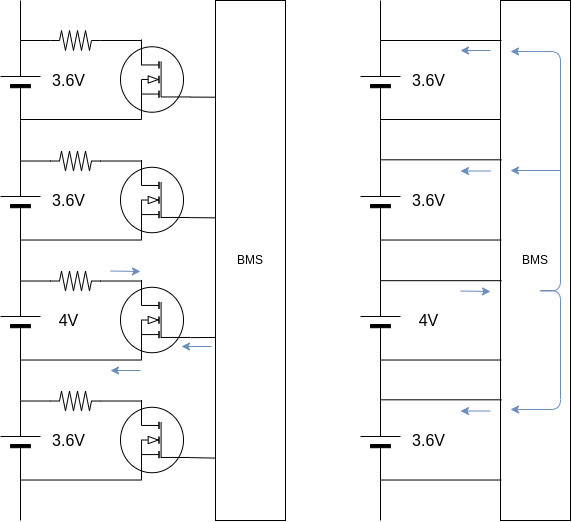
\includegraphics[width=0.7\textwidth]{images/bms-load-balancing.png}
    \caption{Tipos de balanceo de carga. A la izquierda, balanceo pasivo. A la derecha, balanceo activo}
    \label{fig:bms-load-balancing}
\end{figure}

\paragraph{Gestión térmica}
Mantiene a la batería en el rango de operación segura de -10°C hasta 80-85°C, evitando una fuga térmica cuando la temperatura está fuera del rango.  La necesidad de disipar el calor producido por las celdas debido a reacciones electroquímicas es más relevante cuando muchas celdas están agrupadas. En este caso puede utilizarse un sistema de refrigeración activo, como la ventilación forzada.

\paragraph{Evaluación}
Calcula y estima ciertos parámetros relacionados con el estado de la batería.

\begin{itemize}
    \item Estado de carga (SOC)

    Indica la cantidad de energía almacenada utilizable. Permite determinar la carga y descarga óptima y limitar la ventana de operación.

    \item Capacidad

    La capacidad de la batería varía con el tiempo y es el indicador del estado de salud de la celda. Cuando la capacidad se reduce por debajo de cierto límite, la batería llega al fin de su vida útil. Se obtiene descargando la batería en su totalidad a partir de una carga completa.

    $$ Capacidad[Ah] = Intensidad[A] \cdot Tiempo[h] $$

    Existen varios métodos de obtener el SOC como por ejemplo con la tensión de circuito abierto, el conteo de Coulombs, filtros de Kalman, entre otros.

    \item Estado de salud (SOH)

    Se obtiene en base a la capacidad original de la batería y la última capacidad obtenida. La estimación de los parámetros SOC y SOH requieren precisión en los sensores y el desarrollo de complejos algoritmos de estimación.

    \item Tiempo de recarga

    Se estima conociendo la última capacidad obtenida y suponiendo una intensidad de carga constante.

    \item Resistencia interna
    
    Se utiliza para conocer la salud de la batería. Un valor fuera del rango especificado por el fabricante indica que una o varias de las celdas están en mal estado y requieren un reemplazo.
\end{itemize}

\paragraph{Comunicación}
Dependiendo del objetivo del BMS y su construcción, el puerto de comunicación puede ser unidireccional donde los datos a transferir son simples, como la energía restante del sistema, o bidireccional en sistemas más complejos como los buses estandarizados para vehículos eléctricos CAN, RS232, Ethernet, USB, etc. El puerto que soporta el BMS determina la compatibilidad con el resto de las interfaces comunicativas del sistema.

Si bien un BMS incrementa el consumo, costo y la complejidad del sistema, su inclusión es fundamental debido a las numerosas ventajas que presenta:

\begin{itemize}
    \item Descarga uniforme y carga independiente de las celdas en base a su estado.
    \item Permite la operación en su zona segura, estableciendo límites de corriente, tensión y temperatura sobre los cuales se puede esperar que funcione de forma correcta.
    \item Protege la batería mediante desconexión automática en caso de sobre cargas, sobre descargas, sobre corrientes y temperaturas extremas.
    \item Conocer el estado de carga, salud y capacidad de la batería.
    \item Extiende la vida útil de la batería.
    \item Advertencia sobre celdas en mal estado.
    \item Reducción del mantenimiento de la batería.
\end{itemize}